\documentclass[10pt,letterpaper,twoside,notitlepage]{article}
\usepackage[margin=.5in]{geometry}
\usepackage[utf8]{inputenc}
\usepackage{amsmath}
\usepackage{amsfonts}
\usepackage{amssymb}
\usepackage{graphicx}
\usepackage{subfigure}
\author{Karl Hallsby}

\graphicspath{{./Drawings/ECE_211/}}

\begin{document}
\section*{General Equations}
	\begin{itemize}
		\item KCL: $\sum I_{in} = \sum I_{Out}$ \\
			Node's Input Current = Node's Output Current
		\item KVL: $\sum V = 0$ \\
			Voltage across a loop totals to 0.
		\item Conservation of Power: $\sum P = 0$
		\item Power: $P=VI$
		\item Ohm's Law: $V=IR$
	\end{itemize}

\section*{Resistors}
	\begin{itemize}
		\item $V=IR$
		\item Equivalent Series Resistor: $R_{eq} = \sum_{n=1}^{m}R_n$
		\item Equivalent Parallel Resistor: $\frac{1}{R_{eq}} = \sum_{n=1}^{m}\frac{1}{R_n}$
		\item Series Voltage Division: $V_1=\frac{R_1}{R_1+R_2}V_{Source}$
		\item Parallel Current Division: $I_1=\frac{R_2}{R_1+R_2}I_{Source}$
	\end{itemize}

\section*{Methods to Solve Equations}
	\subsection*{Nodal Analysis}
		\begin{enumerate}
			\item \# of Nodes? $\rightarrow n$
			\item Make one node the reference node.
			\item Assign $n-1$ nodal voltages
			\item For a \textbf{voltage} source, write a CONSTRAINT EQUATION (Con. Eq.). If there is a voltage source between 2 non-reference nodes, make that a \textbf{SUPERNODE}.
			\item Write KCL at each node. ($n-1$) equations.
			\item Solve Equations.
		\end{enumerate}
	\subsection*{Mesh/Loop Analysis}
		\begin{enumerate}
			\item \# of Nodes? $\rightarrow n$ \# of Branches? $\rightarrow b$
			\item \# of meshes/loops? $\rightarrow b-n+1 = l$
			\item Assign $l$ loop currents.
			\item For \textbf{current} sources, write a CONSTRAINT EQUATION (Con. Eq.). If there is a current source between 2 meshes, that's a \textbf{SUPERMESH}.
			\item Write KVL for each mesh.
			\item Solve Equations.
		\end{enumerate}

\section*{Source Transformations}
	\textbf{ALL} source transformations obey Ohm's Law. $V=IR$.
	This will \textbf{ONLY} work on resistors in series with \textbf{VOLTAGE} sources, or resistors in parallel with \textbf{CURRENT} sources.
	\begin{figure*}[!htpb]
		\hspace{15mm}
		\begin{subfigure}
			\centering
			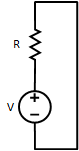
\includegraphics[scale=.4]{SeriesVoltageResistor.png}
			%\caption{Voltage Source in Series with a Resistor}
			\label{fig:SeriesVoltageSource}
		\end{subfigure}
		\hspace{65mm}
		\begin{subfigure}
			\centering
			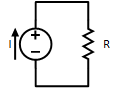
\includegraphics[scale=.4]{ParallelCurrentResistor.png}
			%\caption{Current Source in Parallel with a Resistor}
			\label{fig:ParallelCurrentSource}
		\end{subfigure}
		\caption{Left: Voltage Source in Series with a Resistor, Right: Current Source in Parallel with a Resistor}
	\end{figure*}
\newpage

\section*{Capacitors and Inductors}
	\begin{table}[ht]
		\centering
		\renewcommand{\arraystretch}{1.4}
		\begin{tabular}{|c|c|c|c|}
		\hline
		Relation & R & C & L \\
		\hline
		v-i & $V=IR$ & $v = \frac{1}{C} \int_{t_0}^t i(x)dx + v(t_0)$ & $v=L\frac{di}{dt}$  \\
		i-v & $I=\frac{V}{R}$ & $i = C\frac{dv}{dt}$ & $i=\frac{1}{L}\int_{t_0}^t v(x)dx +i(t_0)$ \\
		\hline
		P or W & $P=I^2R=\frac{V^2}{R}$ & $P=\frac{1}{2}Cv_{c}^2$ & $W=\frac{1}{2}Li_{l}^2$ \\
		\hline
		Series & $R_{eq}=R_1+R_2+\ldots+R_n$ & $\frac{1}{C_{eq}}=\frac{1}{C_1}+\frac{1}{C_2}+\ldots+\frac{1}{C_n}$ & $L_{eq}=L_1+L_2+\ldots+L_n$ \\
		Parallel & $\frac{1}{R_{eq}}=\frac{1}{R_1}+\frac{1}{R_2}+\ldots+\frac{1}{R_n}$ & $C_{eq}=C_1+C_2+\ldots+C_n$ & $\frac{1}{L_{eq}}=\frac{1}{L_1}+\frac{1}{L_2}+\ldots+\frac{1}{L_n}$ \\
		\hline
		@ Steady State & Same (Nothing Happens) & Open Circuit & Short Circuit \\
		\hline
		\end{tabular}
	\end{table}

\section*{Thevenin and Norton Equivalents}
	\begin{itemize}
		\item ONLY independent sources - Zero all sources, find $R_{eq}$.
		\begin{itemize}
			\item 0-ing Current Sources = OC
			\item 0-ing Voltage Sources = SC
			\item Look at circuit from load's perspective for $R_{eq}$
			\item $V_{Th}=V_{OC}$
			\item $I_{N} = I_{SC}$
		\end{itemize}
		\item BOTH dependent and independent sources
			\begin{itemize}
				\item Find $V_{Th}=V_{OC}$
				\item Find $I_{N}=I_{SC}$
				\item Solve $R_{Th}=\frac{V_{OC}}{I_{SC}}$
			\end{itemize}
		\item ONLY dependent sources
			\begin{itemize}
				\item $V_{Th}=0$
				\item $I_{N}=0$
				\item $R_{Th}=R_{N} \rightarrow$ Attach test source @ load.
				\begin{itemize}
					\item If voltage test source, find current
					\item If current test source, find voltage
				\end{itemize}
				\item $R_{Th}=\frac{V}{I}$
			\end{itemize}
		\item \textbf{Maximum Power Transfer} \newline
			$R_{Load}=R_{Th}$ \newline \newline
			$P_{Max}=\frac{V_{Th}^2}{4R_{Th}}$
	\end{itemize}

\section*{Superposition}
	\begin{itemize}
		\item \# of sources, $n$, determines the number of equations you will have.
		\item Shut off each source, one at a time, solving for the term that you want.
		\begin{itemize}
			\item Voltage Source = SC
			\item Current Source = OC
		\end{itemize}
		\item Sum each of the individual terms together. $\sum_{i=1}^{n} x_{i}$
	\end{itemize}
\section*{Solving for RL, RC Circuits}
	\subsection*{Shortcut Method}
		$x(t)=x(\infty )+(x(0)-x(\infty ))e^\frac{-t}{\tau}$, where $x$ could be voltage or current. \newline
		$\tau = RC$ or $\tau = \frac{L}{R}$
	\subsection*{Differential Method}
		\begin{enumerate}
			\item Start by finding the initial value of the voltage across the capacitor or current through the inductor. $t=0^-$, if switch closes at $t=0$.
			\item Use KCL or KVL on the portion of the circuit with the capacitor or inductor. 
			\item Solve the first-order homogenous linear differential equation, with its characteristic equation.
			\item You should end with a solution that is similar to this: $x(t)=K_1e^m + x_s$, where $m$ is the solution to the characteristic equation.
		\end{enumerate}
\section*{Solving for RLC Circuits}
	\subsection*{Shortcut Method}
		$\frac{d^2x}{dt^2}+2\alpha\frac{dx}{dt}+\omega_0^2x=\omega_0^2A_S$ \newline \newline
		$S = -\alpha \pm \sqrt{\alpha^2-\omega_0^2}$ \newline
		There are 3 cases. \newline
		Where $A_S$ is the source, and $K_1$ and $K_2$ are constants that are found:
		\begin{enumerate}
			\item $\alpha > \omega_0 \longrightarrow$ Overdamped \newline
				$x(t)=A_S+K_1e^{S_{1}t}+K_2e^{S_{2}t}$
			\item $\alpha = \omega_0 \longrightarrow$ Critically Damped \newline
				$x(t)=A_S+\left(K_1+K_2t\right)e^{-\alpha t}$
			\item $\alpha < \omega_0 \longrightarrow$ Underdamped \newline
				$x(t)=A_S+\left(K_1\cos(\omega_d t)+K_2\sin(\omega_d t)\right)e^{-\alpha t}$ \\
				$\omega_d=\sqrt{\omega_0^2-\alpha^2}$
		\end{enumerate}
	\subsection*{Differential Method}
		\begin{enumerate}
			\item Start by finding the voltage across the capacitor or current through the inductor. $\left(t=0^-\right)$, this is your first initial condition.
			\item Finding a basic equation for the circuit. $v_R+v_C+v_L=V_S$, or $i_R+i_C+i_L=I_S$.
			\item  Using as an example, $v_R+v_C+v_L=0$.
			\begin{enumerate}
				\item Substitute in what you want to find, using the equations present in the relation table. \newline 
				$L\frac{di}{dt}+\frac{1}{C}\int_{0}^{t}i_{C}(x)dx+v_{C}(0)+iR=V_S$
				\item Find the second initial condition by putting $t=0$ into the above equation, and solving for $\frac{di}{dt}$. \newline
				$L\frac{di}{dt}+\frac{1}{C}\int_{0}^{0}i_{C}(x)dx+v_{C}(0)+iR=0 \longrightarrow L\frac{di}{dt}+\frac{1}{C}(0)+v_C(0)+iR=V_S$
				\item Remove the integral by differentiating the equation. \newline
				$\lbrace L\frac{di}{dt}+\frac{1}{C}\int_{0}^{t}i_{C}(x)dx+v_{C}(0)+iR=V_S\rbrace \frac{d}{dt} \longrightarrow L\frac{d^2i}{dt^2}+\frac{1}{C}i_{C}(t)+R\frac{di}{dt}=0$
				\item Solve the 2nd Order, Linear, Homogenous Differential Equation. (Characteristic Equation $m^2+\frac{R}{L}m+\frac{1}{LC}=0$)\newline
				$\frac{d^2i}{dt}+\frac{R}{L}\frac{di}{dt}+\frac{1}{LC}i=0$
				\item Solving this equation will generate an equation for $i(t)$.\newline
				$i(t)=K_1e^{m_1}+K_2e^{m_2}+I_S$
				\item Solve for $K_1$ and $K_2$ by using the 2 initial conditions you found earlier.
			\end{enumerate}
			\item If you want to find the other half of the equation, voltage across the inductor, or current through a capacitor, use the appropriate relation equation.
		\end{enumerate}
	
\section*{Op Amps}
	\textbf{ONLY} 2 rules: \newline
	The two terminals of the op amp are denoted by the $+$ and $-$.
	\begin{enumerate}
		\item $v^{+}=v^{-}$
		\item $i^{+}=i^{-}=0$
	\end{enumerate}
	%\newpage
	\vspace{3mm} % Some space for the pictures
	
	\begin{figure*}[ht]
		\begin{subfigure}
			\centering
			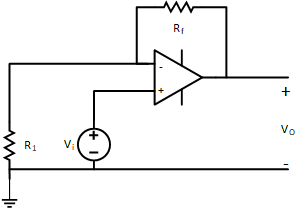
\includegraphics[scale=.7]{NonInvertingAmp.png}
			%\caption{Non-Inverting Amplifier}
			\label{fig:Non-Inverting Amplifier}
		\end{subfigure}
		\begin{subfigure}
			\centering
			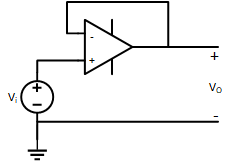
\includegraphics[scale=.7]{Buffer.png}
			%\caption{Buffer}
			\label{fig:Buffer}
		\end{subfigure}
		\hspace{5mm}
		\begin{subfigure}
			\centering
			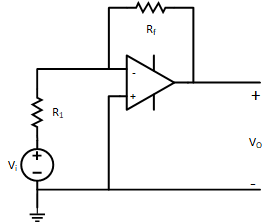
\includegraphics[scale=.7]{InvertingAmp.png}
			%\caption{Inverting Amplifier}
			\label{fig:Inverting Amplifier}
		\end{subfigure}
		\caption{Left: Non-Inverting Amplifier, Middle: Buffer, Right: Inverting Amplifier}
	\end{figure*}
	$V_{O}=\left(1+\frac{R_f}{R_1}\right)V_i$
	\hspace{35mm} $V_{O}=V_{i}$
	\hspace{35mm} $V_{O}=\frac{-R_f}{R_1}V_i, R_f \neq R_1$
	
	\begin{figure*}[ht]
		\begin{subfigure}
			\centering
			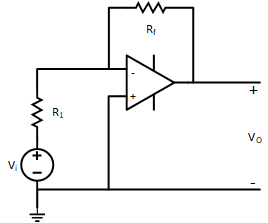
\includegraphics[scale=.7]{Inverter.png}
			%\caption{Inverter}
			\label{fig:Inverter}
		\end{subfigure}
		\hspace{15mm}
		\begin{subfigure}
			\centering
			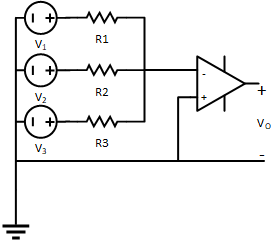
\includegraphics[scale=.7]{Summer.png}
			%\caption{Summer}
			\label{fig:Summer}
		\end{subfigure}
		\hspace{20mm}
		\begin{subfigure}
			\centering
			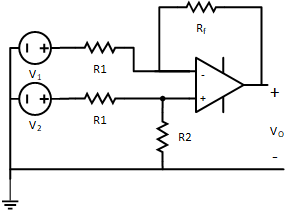
\includegraphics[scale=.7]{Subtractor.png}
			%\caption{Subtractor}
			\label{fig:Subtractor}
		\end{subfigure}
		\caption{Left: Inverter, Middle: Summer, Right: Difference Amplifier}
	\end{figure*}
	$V_{O}=\frac{-R_f}{R_1}V_i, R_f=R_1$
	\hspace{25mm} $V_{O} = -R_f\left(\frac{V_1}{R_1}+\frac{V_2}{R_2}+\frac{V_3}{R_3}\right)$
	\hspace{35mm} $V_{O}=\frac{R_2}{R_1}\left(V_2-V_1\right)$
	
	\begin{figure*}[ht]
		\begin{subfigure}
			\centering
			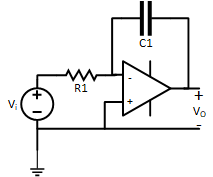
\includegraphics[scale=.7]{Integrator.png}
			%\caption{Integrator}
			\label{fig:Integrator}
		\end{subfigure}
		\hspace{25mm}
		\begin{subfigure}
			\centering
			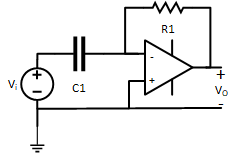
\includegraphics[scale=.7]{Differentiator.png}
			%\caption{Differentiator}
			\label{fig:Differentiator}
		\end{subfigure}
		\caption{Left: Integrator, Right: Differentiator}
	\end{figure*}
	$V_{O}(t)-V_{O}(0)=\frac{-1}{RC}\int_{0}^{t} v_i dt$
	\hspace{30mm} $V_{O}=-R_f C \frac{dv_i}{dt}$
	
\section*{Diodes}
	In an ideal diode, current is only allowed to flow in one direction, the direction of the arrow. \newline
	
	\begin{figure}[!htbp]
		\centering
		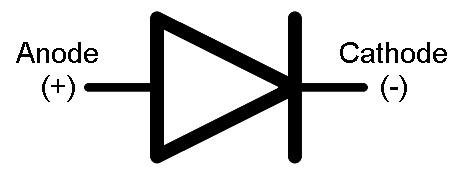
\includegraphics[scale=.15]{Diode.png}
		%\caption{Diode}
		\label{fig:Diode}
	\end{figure} 
	
	In an ideal diode, there are 2 cases:
	\begin{enumerate}
		\item $V_{Anode}-V_{Cathode}>0$ Anode Voltage $>$ Cathode Voltage \newline
			The diode is \textbf{ON}. Current will flow.
		\item $V_{Anode}-V_{Cathode}<0$ Anode Voltage $<$ Cathode Voltage \newline
			The diode is \textbf{OFF}. Current will not flow.
	\end{enumerate}
	
	In reality, a silicon diode needs a $0.7V$ drop across the diode. A germanium diode needs a $0.3V$ drop. 
\end{document}